\subsection{Grafikon kirajzoló - Flot \label{subsec:flot}}

	\begin{figure}[h]
	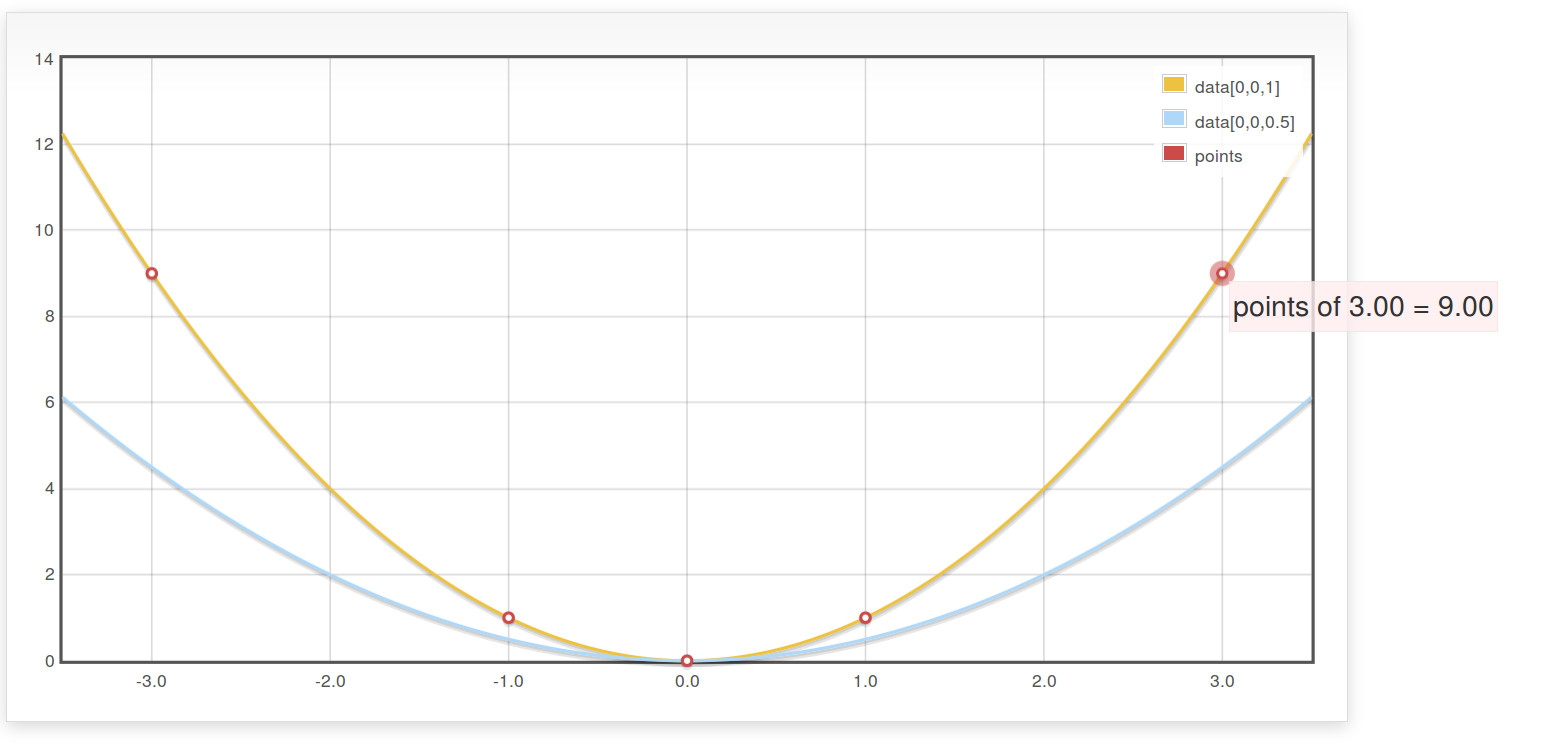
\includegraphics[width=13cm]{pics/plot}
	\centering
	\caption{Grafikon kirajzoló\label{fig:plot}}
	\end{figure}
	
	A Grafikon megjelenítéséhez a Flot 8.0.2-es verzióját használom. Ez egy jQuery-s könyvtár, melyben egyszerűen és látványosan lehet grafikonokat kirajzolni. A forrás a \textit{WebPage/source/flot-8.0.2} mappában érhető el.
	\subsubsection{Felhasználás}
	HTML fájlban egy egyszerű DIV-ként jelenik meg, melyet aztán a JavaScript tölt meg tartalommal.
	\begin{verbatim}
		<div id=\"resultplot\" class=\"demo-placeholder\"></div>
	\end{verbatim}
	A JavaScript-ben hivatkozhatunk erre a \texttt{DIV}-re, majd az adatok és a típusok segítségével alábbi módon hivatkozhatjuk meg: 
	\begin{verbatim}
		var placeholder = $("#resultplot");
		var plot = $.plot(placeholder, flot_data, type);
	\end{verbatim}
	A paraméterezése a grafikon kirajzolónak az alábbi: 
	\begin{description}
		\item[placeholder] \hfill \\ 
 			DIV hivatkozása.
 		 \item[type] \hfill \\ 
 			Megjelenítendő grafikon típusa.
 			\newline
 			A Flot sok lehetőséget nyújt a típusok kiválasztására, és ezekre való példákból megalkottam a saját típusomat mely a következőket tartalmazza egy objektumban:
	 		\begin{verbatim}
				series: { line: { show: true } } 
	 		\end{verbatim}
			Beállítjuk hogy a vonalakat jelenítse meg. Ekkor a pontokat is megjeleníti, a többi beállítás függvényében.
	 		
	 		\begin{verbatim}
				xaxis: { zoomRange: [0.1, 1], panRange: [-1000, 1000] }
				yaxis: { zoomRange: [0.1, 100], panRange: [-1000, 1000] }
	 		\end{verbatim} 
	 		X és Y koordinátákon nagyítás és mozgatási beállítások interaktívvá állítása a xaxis, yaxis elemekkel valósul meg.
		 	\begin{verbatim}
				grid: { hoverable: true, clickable: true }
		 	\end{verbatim} 
		 	Ezeket a tulajdonságokat használjuk arra hogy felvegyünk új pontokat.\newline
		 	Emellett ha ráviszem az egeret az egyik pontra, megmutatja a pont koordinátáját, és értékeit, és hogy melyik ponthalmazon van.
		 	\begin{verbatim}
				zoom: { interactive: true}, pan: { interactive: true }
		 	\end{verbatim} 
		 	Nagyítás és kattintással mozgatás engedélyezése. \newline
			Ennek a beépítésével is foglalkoztam, de a kattintás sajnos nem egyeztethető könnyen össze a pont figyeléssel, valamint a beépítés után lassú lett, és akadozott a felület, így végül az interaktivitását külső komponensekkel(inputokkal) oldottam meg.

 		\item[flot\_data] \hfill \\ 
 		A tényleges adathalmazokat tartalmazó tömb, melyben az egyes adatokról egyéni információkat is tartalmazza.\newline
 		\begin{description}
			\item[data] \hfill \\ 
			Pontok halmaza, melyeket megjelenítünk\newline
			[x, y] pontokból álló tömb\newline
			Polinom esetén is ezt használjuk, ezért a polinom behelyettesített értékeit adjuk itt meg. Amikor az egérrel felé megyünk ezeket a pontokat fogja megjeleníteni.
			\item[label] \hfill \\ 
			Adathalmaz elnevezése, ezt láthatjuk amikor az egérrel a pont felé visszük az egeret, valamint a színek-elnevezések össze párosításánál is segít.
			\item[points] \hfill \\ 
			Ha pontokat kívánunk megjeleníteni, akkor ezt a kapcsolót kell alkalmazni.
			\item[lines] \hfill \\ 
			Ha a pontokból alkotott vonalat kívánunk látni, akkor ezt a kapcsolót kell alkalmazni. Ezt használjuk a polinom megjelenítéséhez.
		\end{description}
 		\begin{verbatim}
		var example_datas = [{
		    data: d4,
		    label: "neved4",
		    lines: { show: true }
		}, {
		    data: d3,
		    label: "neved43"
		    points: { show: true }
		}];
		\end{verbatim}
	\end{description}

\subsection{Http szerver \label{subsec:httpszerver}}
	A szerver kommunikációt Erlang oldalon 2 megtalált minta fájlból állítottam elő. Az egyikben egy egyszerű szerver kommunikációt mutattak be Erlang-ban\cite{simpleserver}. \newline
	A másik pedig az Erlang dokumentációjában megtalálható minta kommunikáció tcp protokollal\cite{tcpserver}.

\subsection{Ping-pong - node figyelő \label{subsec:nodewatcher}}
	http://www.erlang.org/doc/getting\_started/conc\_prog.html
	Az Erlang oldalán található dokumentációban, mely az elosztás és a node kommunikációt mutatja be, sok minta kódot tartalmaz, melyekből könnyen elő tudtam állítani a saját kódomat.\newline
	Ez alapján a párhuzamosítottan számoló programomat könnyen át tudtam alakítani elosztott módon számítóvá. \newline 
	Emellett kellett valami lehetőség arra hogy a gépek fel tudjanak csatlakozni a szerverre. Lehetőség lett volna arra is hogy a figyelő helyett csak megkapja a gépek listáját a szerver, de így tisztábban szét van választva a háttér és a kliens, és nem is szükségesek a tényleges számításhoz. \newline
	Ezen az oldalon található minták a ping-pong kommunikációra, melynek segítségével hoztam létre a node-figyelőt. Ez a modul a \texttt{ServerConfig/nodeWatcher.erl} fájlban található meg. \newline

	Ennek mintájára hoztam létre az alábbi figyelőt, melyet regisztrálunk \texttt{pid\_watcher} atom segítségével. 
	\begin{verbatim}
	startPidWatch() ->
	    PidWatch = spawn(nodeWatcher, pidWatch, [self(), []]),
	    register(pid_watcher, PidWatch),
	    PidWatch.
	\end{verbatim}

	A másik gépről ezután lehet küldeni egy \textit{"ping"}-et, melyet megkap a node-figyelő.
	\begin{verbatim}
	registerToServer(Pong_Node) ->
	    spawn(nodeWatcher, registerToServerNode, [Pong_Node]).
	...
	registerToServerNode(Pong_Node) -> 
	    {pid_watcher, Pong_Node} ! {worker_write, self(), node()},
	    ...
	\end{verbatim}


\subsection{Struktúra kezelő - mochijson \label{subsec:mochijson}}
	A mochijson egy Erlang-hoz is használt modul, melynek segítségével egy json string-et át lehet konvertálni Erlang-os struktúrává. \newline 
	\texttt{git clone https://github.com/mochi/mochiweb.git}(2015.05)
	paranccsal a teljes mochiweb könyvtárat le lehet tölteni. A \texttt{mochiweb/src} mappában találhatóak azok a fájlok melyeket le lehet fordítani, és be lehet tölteni az Erlang shell-be. Lehet letölteni a fájlokat különállóan is. \newline
	Eredetileg csak a mochijson.erl-re volt szükségem, de miután komplexebb adatot kellett encode-olnom szükségessé vált még egy fájl betöltése, viszont nem tudtam hogy az még milyen függőségeket hordoz magában, így letöltöttem az egész repository-t. \newline
	Ha Erlang-ban lefordítjuk shell-ben \texttt{mochijson:encode, decode} függvényekkel egyszerűen lehet használni.\newline 
	Példa képen megtekinthetjük az alábbi egyszerű json-t, mely már tartalmaz objektumot és tömböt.
	\begin{verbatim}
		{
		    "1": {
		        "result": [
		            0.1,
		            0.5,
		            0.7
		        ],
		        "time": 0.5
		    }
		}
	\end{verbatim}
	Ennek string formájára meghívhatjuk a mochijson decode függvényt.
	\begin{verbatim}
	ErlStruct = mochijson:decode(
	    "{\"1\":{\"result\":[0.1,0.5,0.7],\"time\":0.5}}"
	).
	\end{verbatim}
	Ennek eredménye egy Erlang-os struktúra.
	\begin{verbatim}
		{struct, [
		    {"1", {struct,[
		          {"result",{array,[0.1,0.5,0.7]}},
		          {"time",0.5}
		    ]}}
		]}
	\end{verbatim}
	Az \texttt{mochijson:encode} segítségével pedig ezt a struktúrát vissza tudjuk alakítani json string-gé. Bár az eredményt shell-ben binary formában lehet egyszerűen megtekinteni, és ebben a formában is kell visszaküldeni a kliensnek. 
	\begin{verbatim}
		iolist_to_binary(mochijson:encode(ErlStruct)).
		<<"{\"1\":{\"result\":[0.1,0.5,0.7],\"time\":0.5}}">>
	\end{verbatim}


	\subsubsection{Felhasználás}
	Ennek a típusa nem egyszerű, főleg ilyen komplex adathalmaznál. Ennek kezelésére létre lett hozva a \texttt{Utility/structHandler} modul. \newline 
	Első lépésben a string-et konvertáljuk a kellő típussá. 
	\begin{verbatim}
		getDataByJson(JsonSting) -> apply(mochijson, decode, [JsonSting]).
	\end{verbatim}
	Ismeretek segítségével létre hoztam egy olyan függvényt, ami kinyer egy adott értéket a struktúrából.
	\begin{verbatim}
		getElementByKey(array, {array, Array}) -> Array;
		getElementByKey(struct, {struct, Array}) -> Array;
		getElementByKey(Name, {struct, Struct}) -> 
		    getElementByKey(Name, Struct);
		getElementByKey(Name,[{Name, Value}]) -> Value;
	\end{verbatim}
	Ennek felhasználásával dolgoztam fel a struktúrát.

\subsection{\label{subsec:nif} Erlang modul C++-ban - NIF}

	NIF \cite{erl_nif} (native implemented functions) egy C könyvtár, melynek segítségével implementálhatjuk egy modul függvényeit C-ben vagy C++-ban. 
	\subsubsection{Felhasználás}
	A calculator Erlang-modul megvalósítását C++-ban implementáltuk.\newline
	\texttt{Calculator/} mappában található \texttt{erlang.cpp} és a \texttt{calculator.erl} fájlokban használjuk fel a NIF-et.
	Amely fájlban végezzük a modul közvetlen kommunikációját az Erlang-al ott le kell tölteni az \texttt{erl\_nif} könyvtárat.
	\begin{verbatim}
		#include "erl_nif.h"
	\end{verbatim}
	Emellett meg kell neki adni, melyik függvényeket, hány paraméterrel szeretnénk az Erlang-ba betölteni. 
	A fájlt \texttt{Calculator/erlang.cpp} néven találhatjuk meg.
	\begin{verbatim}
		static ErlNifFunc nif_funcs[] = {
		    {"calculate", 4, calculate_nif}
		};
	\end{verbatim}
	Amikor inicializáljuk, le kell írni hogy melyik modul-nak lesz a része. 
	\begin{verbatim}
		ERL_NIF_INIT(calculator, nif_funcs, NULL, NULL, NULL, NULL)
	\end{verbatim}
	Amikor meghívódik az Erlang-ból ez a modul, paraméterként \texttt{ERL\_NIF\_TERM} típusú változókat kapunk, melyeket lehetőség van átkonvertálni C++-os típusokká. \newline
	Az \texttt{enif\_get\_int} függvény segítségével egy változóból kinyerhetjük az integer-ré konvertált értéket. Hasonlóan használjuk az \texttt{enif\_get\_double} függvényt mely értelemszerűen egy double típusú értéket ad vissza.
	\newline
	Egy lista elemeit \texttt{enif\_get\_list\_cell} függvény segítségével tudtam átkonvertálni. 
	Ennek segítségével megvalósítottam a vektor-rá és mátrix-á átalakító függvényeket,
	\begin{verbatim}
		ERL_NIF_TERM head; ERL_NIF_TERM tail = arg;
		//...
		while(enif_get_list_cell(env, tail, &head, &tail)) {
		    //...
		}
	\end{verbatim}
	A számítás eredménye egy vektor, így az eredményül kapott értéket vissza kell valahogyan konvertálni Erlang-os típussá. Ezt az \texttt{enif\_make\_double} és az \\ \texttt{enif\_make\_list\_from\_array} függvények segítségével lehet megvalósítani. 
	Ennek implementálása a \texttt{convertList} függvényben történt.
	\newline
	A tényleges híváshoz a \texttt{nif\_funcs}-ban meghivatkozott \texttt{calculate\_nif}-et kell implementálni. \newline
	Ebben meghívódnak a konvertáló függvények a helyes paraméterezés kialakításához, majd az eredménnyel visszatérünk egy lista formájában.
	\begin{verbatim}
	static ERL_NIF_TERM calculate_nif
	(ErlNifEnv* env, int argc, const ERL_NIF_TERM argv[]) {
	    //...
	    poli = interpolateMain(X, Y, type, isInverse);
	    return convertList(env, poli);
	}
	\end{verbatim}

\subsection{Dokumentációhoz felhasznált programok}
	A tervezési, és megvalósítási szemléltető képek és diagramok egy webes szerkesztő segítségével valósultak meg. Ez az oldal 2015-ben a http://creately.com/ címen volt elérhető.